\documentclass[aspectratio=34]{beamer}

\usepackage{polyglossia}
\setmainlanguage{english}

\usepackage{fontspec}
\setsansfont{Arial}

\usetheme{epiukbonn}

\usepackage{shadowtext}
\shadowoffset{1pt}
\shadowcolor{black}
\definecolor{epitalktitlecolor}{HTML}{FF6600}
\definecolor{epispeakercolor}{HTML}{FFFF00}


\newcommand{\lineoftitle}[1]{\shadowtext{\color{epitalktitlecolor} \LARGE \textbf{#1}}} 


\begin{document}

% This is a sample title page
\begin{frame}{}
  \begin{center}
   \begin{tikzpicture}[every text node part/.style={align=center}]
    \node[inner sep = 0pt] (a) {\frame{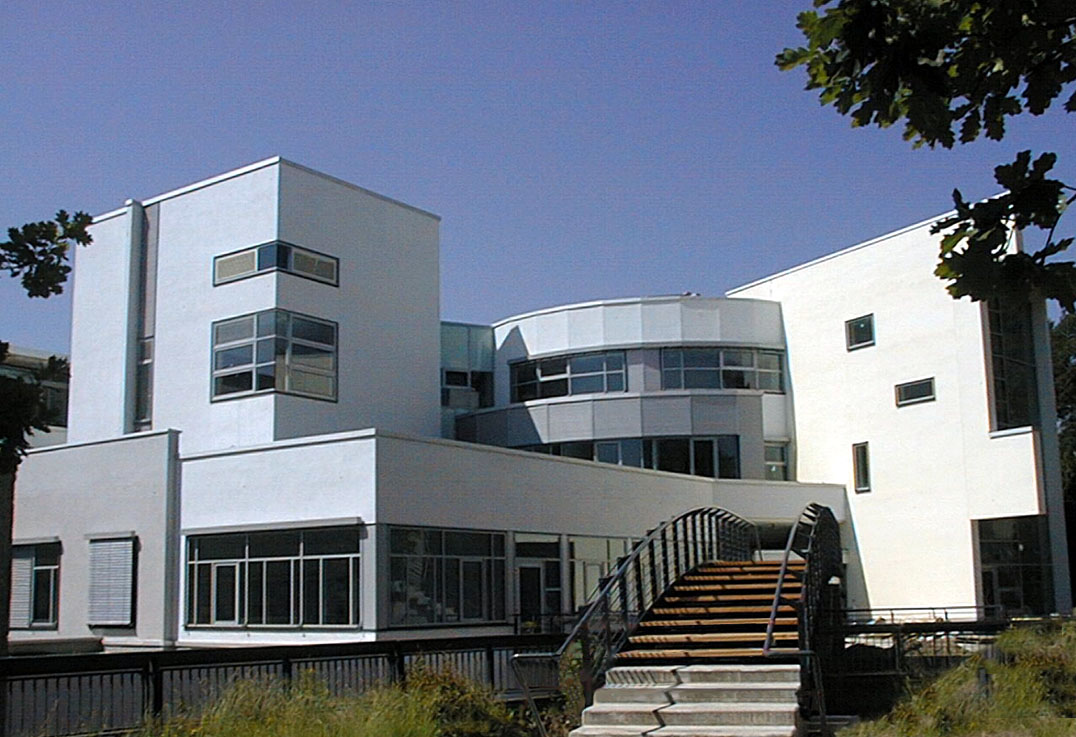
\includegraphics[width=.8\textwidth]{../figures/building_epi.jpg}}};
    \node[anchor=center, inner sep=1pt, shift={(0em,3.5em)}] at (a.center) {
      \color{epitalktitlecolor}
      \lineoftitle{Reactivation of concept cells}\\[.3em]
      \lineoftitle{in the human brain}\\[.3em]
      \lineoftitle{during sleep}\\[.3em]
      \lineoftitle{after episodic learning}};

    \node[anchor=center, inner sep=1pt, shift={(0em,-3em)}] at (a.center) {
      \color{epispeakercolor}
      \shadowtext{\color{epispeakercolor}\Large Johannes Niediek}};
  \end{tikzpicture}
  \begin{tikzpicture}[remember picture,overlay]
 \node [xshift=0cm,yshift=0cm] at (current page.south west)
    [above right]
    {\tiny \textit{www.epileptologie-bonn.de}};
      \end{tikzpicture}
    \end{center}

\end{frame}

% This is a sample normal page
\begin{frame}{Background: \textbf{Memory consolidation}}
  \begin{block}{}
    \begin{itemize}
    \item Patient H.\,M.
    \item Place cells in rodents
      \end{itemize}
    \end{block}
    
\end{frame}

\end{document}